\documentclass[12pt,a4paper,draft]{article}
%setting margins
\usepackage[margin=0.75in]{geometry}


%%%%%%%%%%%%%%%%%%%%%%%%%%%%%%%%%%%%%%%%%%%%%%%%%%%%%%%%
%packages
\usepackage{amsmath}
\usepackage{amsthm}
\usepackage{blindtext}
\usepackage{fancyhdr}
\usepackage{enumerate}
\usepackage[shortlabels]{enumitem}
\usepackage{setspace}
\usepackage{tcolorbox}
\usepackage{pgfplots}
\usepackage{multicol}
\usepackage{subfiles} % Best loaded last in the preamble
\pgfplotsset{compat=1.18}
\usepackage{subcaption}
\usepackage{graphicx}
\usepackage{tabularray}
\usepackage{circuitikz}

\usepackage[thinc]{esdiff}
%%%%%%%%%%%%%%%%%%%%%%%%%%%%%%%%%%%%%%%%%%%%%%%%%%%%%%%%
\pagestyle{fancy}
\fancyhead[l]{Rüzgar Erik}
\fancyhead[c]{Notes For the 13th Unit}
\fancyhead[r]{MATH104}
\fancyfoot[c]{\thepage}
\renewcommand{\headrulewidth}{0.2pt}
\setlength{\headheight}{15pt}
%%%%%%%%%%%%%%%%%%%%%%%%%%%%%%%%%%%%%%%%%%%%%%%%%%%%%%%%
%makes all equations centered use originalequation for normal mode
\let\originalequation\equation
\let\endoriginalequation\endequation

\renewenvironment{equation}
  {\begin{center}\originalequation}
  {\endoriginalequation\end{center}}


%%%%%%%%%%%%%%%%%%%%%%%%%%%%%%%%%%%%%%%%%%%%%%%%%%%%%%%%
%Define a new tcolorbox environment named "definition"
  \newtcolorbox{definitionbox}{
    colback=blue!5!white,
    colframe=blue!75!black,
    title=DEFINITION(S)
  }
  
  \newenvironment{definition}{\begin{definitionbox}}{\end{definitionbox}\vspace{1\baselineskip}}

%%%%%%%%%%%%%%%%%%%%%%%%%%%%%%%%%%%%%%%%%%%%%%%%%%%%%%%%
\newcommand{\example}{\vspace{1\baselineskip}\par\noindent\textcolor{red}{\textbf{EXAMPLE}: }}
\newcommand{\solution}{\par\noindent\textcolor{red}{\textbf{SOLUTION}: }\vspace{1\baselineskip}}

%%%%%%%%%%%%%%%%%%%%%%%%%%%%%%%%%%%%%%%%%%%%%%%%%%%%%%%%

%Define a new tcolorbox environment named "theorem"
\newtcolorbox{theorembox}[1]{
    colback=red!5!white,
    colframe=red!75!black,
    title=THEOREM
  }
  
  \newenvironment{theorem}{\begin{theorembox}}{\end{theorembox}\vspace{1\baselineskip}}

%%%%%%%%%%%%%%%%%%%%%%%%%%%%%%%%%%%%%%%%%%%%%%%%%%%%%%%%

\newtcolorbox{corollarybox}{
    colback=blue!5!white,
    colframe=blue!75!black,
    title=Corollary
}
  
\newenvironment{corollary}{\begin{corollarybox}}{\end{corollarybox}\vspace{1\baselineskip}}


\newtcolorbox{rulebox}[1]{
    colback=red!5!white,
    colframe=red!75!black,
    title=#1
}

\newenvironment{ruleBox}[1]{\begin{rulebox}{#1}}{\end{rulebox}\vspace{1\baselineskip}}


%%%%%%%%%%%%%%%%%%%%%%%%%%%%%%%%%%%%%%%%%%%%%%%%%%%%%%%%

%Define a new tcolorbox environment named "theorem"

\newtcolorbox{note}{
    colback=white,
    colframe=black,
}

\newenvironment{mynote}{\vspace{1\baselineskip}\begin{note}}{\end{note}\vspace{1\baselineskip}}

%%%%%%%%%%%%%%%%%%%%%%%%%%%%%%%%%%%%%%%%%%%%%%%%%%%%%%%%



\newcommand{\lopital}{L'Hôpital's Rule }
\newcommand{\anc}{\(\{a_n\}\)}
\newcommand{\fxy}{\(f(x,y)\)}
\newcommand{\an}{\(a_n\)}

\newcommand{\infsum}{\sum_{n=1}^{\infty}}
\fancypagestyle{firstpage}{
    \fancyhf{} % Clear header and footer
    \renewcommand{\headrulewidth}{0pt} % Remove header rule
}

% Redefine \maketitle to include a fancy box
\makeatletter
\renewcommand{\maketitle}{%
  \thispagestyle{firstpage} % Apply the firstpage style for the first page
  \begin{tcolorbox}[colback=white,colframe=black,width=\textwidth,arc=0mm,auto outer arc]
    \begin{center}
      \Large \@title \\[1ex] \large \@date \\ \textit{Rüzgar ERİK}
    \end{center}
  \end{tcolorbox}
}
\makeatother

\usepackage{parskip}
\setlength{\parindent}{0pt} % Disable paragraph indentation


\usepackage{hyperref}
\hypersetup{
    colorlinks,
    citecolor=black,
    filecolor=black,
    linkcolor=black,
    urlcolor=black
}


%%%%%%%%%%%%%%%%%%%%%%%%%%%%%%%%%%%%%%%%%%%%%%%%%%%%%%%%
\begin{document}



\title{Partial Derivatives}
\date{MATH 104}
\maketitle
\tableofcontents % This command generates the index page

\newpage % Start a new page for the content

\section{Partial Derivatives}
\subsection{Functions of Several Variables}

Real-valued functions of several independent real variables are defined analogously to functions of a single variable. Points in the domain are now ordered pairs of real numbers, and values in the range are real numbers.

\begin{definition}
    Suppose \textit{D} is a set of n-tuples of real numbers \(x_1, x_2, \dots, x_n\).
    A \textbf{real-valued function} \(f\) on \textit{D} is a rule that assigns a unique real numbers
    \[w = f(x_1, x_2, \dots, x_n)\]
    to each element in \textit{D}. The set \textit{D} is the function's \textbf{domain}. The set of w-values taken on by \(f\) is the function's \textbf{range}. The symbol w is the \textbf{dependent variable} of \(f\) and \(f\) is said to be a function of the n \textbf{independent variables} \(x_1\) to \(x_n\).
    We also call \(x_j\)'s the function's \textbf{input variables} and call w the function's \textbf{output variable}.

\end{definition}


\noindent If \(f\) is a function of two independent variables, we usually call the independent variables x and y and dependent variable z, and we picture the domain of f as a region in the xy-plane.
If \(f\) is a function of three independent variables, we call the independent variables x, y and z and the dependent variable w, and we picture the domain as a region in space.



%\newpage

\subsection{Domains and Ranges}

\noindent If defining a function of more then one variable, we follow the usual practice of excluding inputs that lead to complex numbers or division by zero. If \(f(x,y) = \sqrt{y - x^2}\) then y cannot be less than \(x^2\).
If \(f(x,y) = 1\slash (xy)\) then xy cannot be zero. 


\begin{example}

    \noindent These are functions of two variables. Note the restrictions that may apply to their domains in order to obtain a real value for the dependent variable \( z \).

    \begin{table}[h]
        \centering
        \begin{tblr}{
          width = \linewidth,
          colspec = {Q[304]Q[190]Q[448]},
          hline{1,5} = {-}{0.08em},
          hline{2} = {-}{},
        }
        \textbf{Function}    & \textbf{Domain} & \textbf{Range}                  \\
        \( z = \sqrt{y - x^2} \) & \( y \geq x^2 \)    & \( [0, \infty) \)                   \\
        \( z=\frac{1}{xy} \)     & \( xy \neq 0 \)     & \( (-\infty, 0) \cup (0, \infty) \) \\
        \( z = \sin(xy) \)       & Entire Plane    & \( [-1,1] \)                        
        \end{tblr}
    \end{table}
    
    \noindent These are functions of three variables with restrictions on some of their domains.
    
    \begin{table}[h]
        \centering
        \begin{tblr}{
          width = \linewidth,
          colspec = {Q[304]Q[250]Q[448]},
          hline{1,5} = {-}{0.08em},
          hline{2} = {-}{},
        }
        \textbf{Function}    & \textbf{Domain} & \textbf{Range}                  \\
        \( z = \sqrt{x^2 + y^2 + z^2 } \) & Entire space    & \( [0, \infty) \)                   \\
        \( z=\frac{1}{x^2 + y^2 + z^2} \)     & \( (x, y, z) \neq (0,0,0) \)     & \( (0, \infty) \) \\
        \( z = xy \ln(z) \)       & Half space \(z > 0\)    & \( (- \infty,\infty) \)                        
        \end{tblr}

    \end{table}

\end{example}

\newpage


\subsection{Functions of Two Variables}

Regions in the plane can have interior points and boundary points kust like intervals on the real line.
Closed intervals \([a, b]\) include their boundary points, open intervals \((a,b)\) don't include their boundary points and intervals such as \([a,b)\) are neither open nor closed.

\begin{definition}
    A point \((x_0, y_0)\) in a region (set) \(R\) in the xy-plane is an \textbf{interior point} of \(R\) if it is the center of positive radius that lies entirely in \(R\).
    A point \((x_0, y_0)\) is a \textbf{boundary point} of \(R\) if every disk centered at \((x_0, y_0)\) contains point that lşe outside of \(R\)  as well as points that lie in \(R\). (The boundary point need itself need not belong to \(R\)).
    The interior points of a region, as a set, make up the \textbf{interior} of the region. The region's boundary points make up its \textbf{boundary}.
    A region is \textbf{open} if it contains entirely of interior points. A region is \textbf{closed} if it contains all its boundary points.

\end{definition}



\begin{figure}[h!]
    \centering
    
    \begin{minipage}[t]{0.3\textwidth}
        \centering
        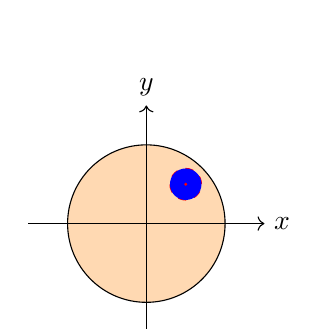
\begin{tikzpicture}
            \fill[orange!30] (0,0) circle (1);
            \draw[->] (-1.5,0) -- (1.5,0) node[right] {$x$};
            \draw[->] (0,-1.5) -- (0,1.5) node[above] {$y$};
            \draw (0,0) circle (1);
            \draw[dashed, red] (0.5,0.5) circle (0.2);
            \fill[blue] (0.5,0.5) circle (0.2);
            \fill[red] (0.5,0.5) circle (0.02);
        \end{tikzpicture}
        \caption{ \(\{(x,y) | x^2 + y^2 < 1\}\) Open unit disk. Every point an interior point.}
        \label{fig:first}
    \end{minipage}
    \hfill
    \begin{minipage}[t]{0.3\textwidth}
        \centering
        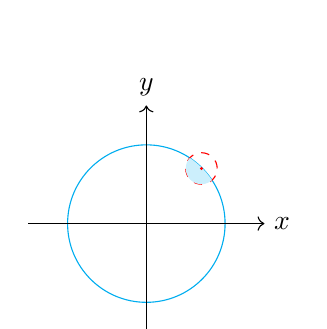
\begin{tikzpicture}
            \draw[cyan] (0,0) circle (1);
            \draw[->] (-1.5,0) -- (1.5,0) node[right] {$x$};
            \draw[->] (0,-1.5) -- (0,1.5) node[above] {$y$};
            \draw[dashed, red] (0.7,0.7) circle (0.2);
            \begin{scope}
                \clip (0,0) circle (1);
                \fill[cyan!20] (0.7,0.7) circle (0.2);
            \end{scope}
            \fill[red] (0.7,0.7) circle (0.02);
        \end{tikzpicture}
        \caption{ \(\{(x,y) | x^2 + y^2 = 1\}\) Boundry of unit disk.}
        \label{fig:second}
    \end{minipage}
    \hfill
    \begin{minipage}[t]{0.3\textwidth}
        \centering
        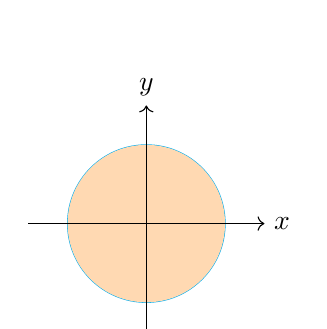
\begin{tikzpicture}
            \draw[cyan] (0,0) circle (1);
            \fill[orange!30] (0,0) circle (1);
            \draw[->] (-1.5,0) -- (1.5,0) node[right] {$x$};
            \draw[->] (0,-1.5) -- (0,1.5) node[above] {$y$};
        \end{tikzpicture}
        \caption{ \(\{(x,y) | x^2 + y^2 \leq 1\}\) Closed unit disk. Contains all boundary points.}
        \label{fig:third}
    \end{minipage}

    \vspace{1\baselineskip}


\end{figure}

\noindent As with a half-open interval of real numbers \([a,b)\), some regions in the plane are neither open nor closed. If you start with the open disk Figure \ref{fig:second} and add to it some, but not all, of its boundary points, the resulting set is neither open nor closed. The boundary points that \textit{are} there keep the set from being open. The absence of the remaining boundary points keeps the set from being closed. Two interesting examples are the empty set and the entire plane. The empty set has no interior points and no boundary points. This implies that the empty set is open and at the same time it is closed. The entire xy-plane is also both open and closed: open because every point in the plane is an interior point, and closed because it has no boundary points. The empty set and the entire plane are the only subsets of the plane that are both open and closed.

\begin{definition}
    A region in the plane is \textbf{bounded} if it lies inside a disk of finite radius. A region is \textbf{unbounded} if it is not bounded.
    
\end{definition}
Examples of \textit{bounded} sets in the plane include line segments, triangles, interiors of triagles, rectangles, circles and disks. Examples of \textit{unbounded} sets in the plane include, lines, coordinate axes, the graphs of functions defined on infinite intervals, quadrants, half-planes, and the plane itself.

\newpage


\begin{example}
    Describe the domain of the function \(f(x,y)=\sqrt{y-x^{2}}\).
    \begin{figure}[h]
        \centering
        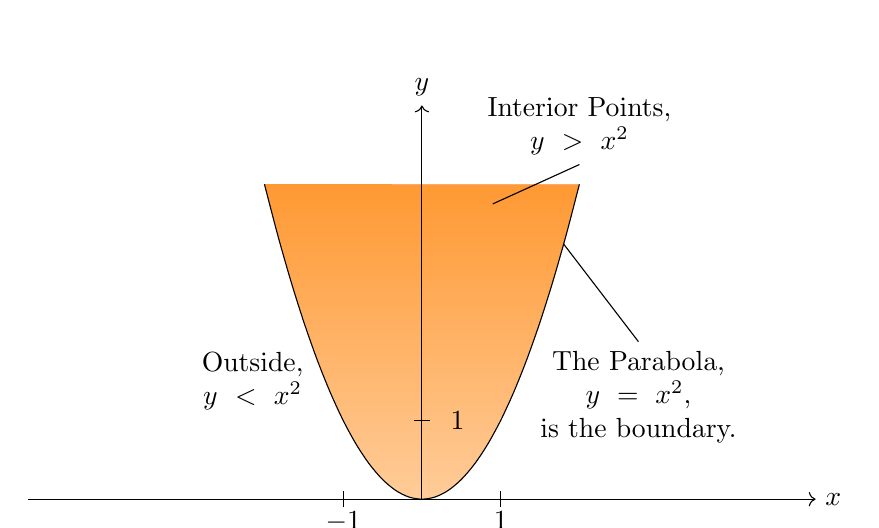
\begin{tikzpicture}
            % Draw the curve y = x^2
            % Fill the area under the curve with 30% orange
            \pgfdeclareverticalshading{parabolashading}{100bp}{color(0bp)=(orange!20); color(100bp)=(orange)}
            \fill[purple!30, domain=-2:2, variable=\x, shading=parabolashading] plot ({\x},{\x*\x}) -- cycle;
            % Draw axes and ticks
            \draw[->] (-5,0) -- (5,0) node[right] {$x$};
            \draw[->] (0,0) -- (0,5) node[above] {$y$};
            \draw (1,-0.1) -- (1,0.1) node[below=4pt] {$1$};
            \draw (-1,-0.1) -- (-1,0.1) node[below=4pt] {$-1$};
            \draw (-0.1,1) -- (0.1,1) node[right=4pt] {$1$};
            % Draw the parabola
            \draw[domain=-2:2, smooth, variable=\x] plot ({\x},{\x*\x});
            % Add labels and pointers
            \node[text width=3cm, align=center] at (-2.15,1.5) {Outside, \\ $y < x^2$}; % Text
            \draw[-] (0.9,3.75) -- (2,4.25); % Pointer
            \node[text width=3cm, align=center, anchor=south] at (2,4.25) {Interior Points, \\ $y > x^2$}; % Text
            \draw[-] (1.8,3.24) -- (2.75,2); % Pointer
            \node[text width=3cm, align=center, anchor=north] at (2.75,2) {The Parabola, \\ $y = x^2$, \\ is the boundary.}; % Text
        \end{tikzpicture}
        \caption{The domain of $f(x, y)$ in this example consists of the shaded region and its bounding parabola.}
        \label{fig:parabola1}
    \end{figure}
    
\end{example}


\begin{solution}

    Since \(f\) is defined only where \(y - x^2 \geq 0\), the domain is the closed unbounded region shown in Figure \ref{fig:parabola1}. The parabola \(y = x^2\) is the boundry of the domain. The points above the parabola make up the domain's interior. \hfill \qed
\end{solution}

\subsection{Graphs, Level Curves, and Contours of Functions of Two Variables}

There are two standard ways to picture the values of a function \(f(x,y)\). One is to draw and label curves in the domain on which \(f\) has a constant value. The other is to sketch the surface \(z\ =\ f(x,y)\) in space.

\begin{definition}
    The set of points in the plane where a function \(f(x,y)\) has a constant value \(f(x,y) = c\) is called a \textbf{level curve} of \(f\).
    The set of all points \((x, y, f(x,y))\) in soace for \((x,y)\) in the domain of \(f\) is called the \textbf{graph} of \(f\).
    The graph of \(f\) is also called the \textbf{surface} \(\mathbf{z = f(x,y)}\).
\end{definition}

\newpage

\begin{example}
    Graph \(f(x,y) = 100 - x^2 - y^2\) and plot the level curves \(f(x,y) = 0\), \(f(x,y) = 51\), \(f(x,y) = 75\) in the domain of f in the plane.
    \begin{figure}[h]
        \centering
        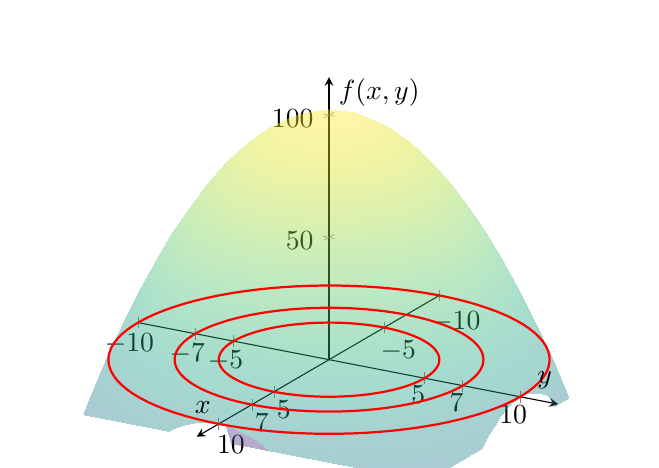
\begin{tikzpicture}
            \begin{axis}[
                xlabel={$x$},
                ylabel={$y$},
                zlabel={$f(x,y)$},
                domain=-10:10,
                y domain=-10:10,
                samples=40,
                view={120}{30},
                axis lines=center,
                width=10cm,
                height=8cm,
                zmin=0,
                zmax=105,
                enlargelimits=upper,
                xtick={-10,-5,5,7,10},
                ytick={-10,-7,-5,5,7,10},
                grid=none,
                colormap/viridis
                ]
                
                \addplot3[surf,opacity=0.4,shader=interp] {100 - x^2 - y^2}; 
                \addplot3[domain=0:360, samples=100, samples y=0, red, thick] ({10*cos(x)}, {10*sin(x)}, {0});
                \addplot3[domain=0:360, samples=100, samples y=0, red, thick] ({7*cos(x)}, {7*sin(x)}, {0});
                \addplot3[domain=0:360, samples=100, samples y=0, red, thick] ({5*cos(x)}, {5*sin(x)}, {0});


            \end{axis}
        \end{tikzpicture}

        \caption{Surface plot of $f(x,y) = 100 - x^2 - y^2$ .}
        \label{fig:surfaceplot}
    \end{figure}

\end{example}

\begin{solution}
    The domain of \(f\) is the entire xy-plane, and the range of \(f\) is the set of real numbers less than or equal to 100. The graph is the paraboloid \(z = 100 - x^2 - y^2\), the positive portion which is shown in Figure \ref{fig:surfaceplot}. \\
    The level curve \(f(x,y) = 0\) is the set of points in the xy-plane at which
    \[f(x,y) = 100 - x^2 - y^2 = 0 \quad \text{or} \quad x^2 + y^2 =100\],
    which is the circle of radius 10 centered at the origin. Similarly the level curves \(f(x,y) = 51\) and \(f(x,y) = 75\) are the circles
    \begin{align*}
        f(x,y) &= 100 - x^2 - y^2 = 51 \quad \mathtt{or}  \quad x^2 + y^2 = 49 \\
        f(x,y) &= 100 - x^2 - y^2 = 75  \quad \mathtt{or}  \quad x^2 + y^2 = 25
    \end{align*}
    
    The level curve \(f(x,y) = 100\) consists of the origin alone. \\
    If \(x^2 + y^2 > 100\) then the values of \(f(x,y)\) are negative. For example the circle \(x^2 + y^2 = 144\), which is the circle centered at the origin with radius 12, gives the constant value \(f(x,y) = -44\) and is a level curve of \(f\). \hfill \qed

    The curve in space in which \(z = c\) cuts a surface \(z = f(x,y)\) is made up of the points that represent the function value \(f(x,y) = c\). It is called the \textbf{contour curve} \(f(x,y) =c\) to distinguish from the level curve \(f(x,y) =c\) in the domain of \(f\). \\
    \textcolor{red}{\textbf{Contour curves lie on the plane z = c, level curves are the projections to the xy-plane}}

\end{solution}

\newpage
\subsection{Functions of Three Variables}

In the plane, the points where a function of two independent variables has a constant value \(f(x,y) =c\) make a curve in the functions domain. In space the poins where a function of three variables has a constant value \(f(x,y,z) =c\) make a surface in the function's domain.

\begin{definition}
    The set of points \((x,y,z)\) in space where a function of three independent variables has a constant value \(f(x,y,z) =c\) is called a \textbf{level surface} of \(f\).
\end{definition}

\begin{example}
Describe the level surfaces of the function
\[f(x,y,z)=\sqrt{x^{2}+y^{2}+z^{2}}\]
\end{example}

\begin{solution}
    The value of \(f\) şs the distance from origin to the point \((x,y,z)\). 
    Each level surface \(\sqrt{x^{2}+y^{2}+z^{2}} = c\), \(c>0\), is a sphere of radius c centered at the origin.
\end{solution}

\begin{definition}
    A point \((x_0,y_0,z_0)\) in a region \textit{R} in space is an \textbf{interior point} of \textit{R} if it is the center of a solid ball that lies entirely in \textit{R}. 
    A point \((x_0,y_0,z_0)\) is a \textbf{boundary point} of \textit{R} if every solid ball centered at \((x_0,y_0,z_0)\) contains points that lie outside of \textit{R} as well as points that lie inside \textit{R}.
    The \textbf{interior} of \textit{R} is the set of interior points of \textit{R}. The \textbf{boundary} of \textit{R} is the set of boundary points of \textit{R}.\\
    A region is open if it consists \textbf{entirely of interior points}. A region is \textbf{closed} if it contains its entire boundary.

\end{definition}

Examples of \textit{open sets} in space include the interior of a sphere, the open half-space \(z > 0\), the first octant, and the space itself. 
Examples of \textit{closed sets} in space include lines, planes, and closed half space \(z \geq 0\). A solid sphere with part of its boundary removed or a solid cube with a missing face, edge, or corner point is \textit{neither open nor closed}.

\newpage 

\section{Limits and Continuity in Higher Dimensions}

If the values of \(f(x,y)\) lie arbitrarily close to a fixed real number \textit{L} for all points \((x,y)\) sufficiently close to a point \((x_0,y_0)\), we say that \(f\) approaches the limit \textit{L} as \((x,y)\) approaches \((x_0,y_0)\).
This is similar to the informal definition for the limit of a function of a single variable. Notice, however, then when \((x_0,y_0)\) lies in the interior of \(f\)'s domain, \((x,y)\) can approach \((x_0,y_0)\) from any direction, not just from the left or the right. For the limit to exist, the same limiting value must be obtained whatever direction of approach is taken.

\begin{definition}
    We say that a function \(f(x,y)\) approaches the \textbf{limit} \textit{L} as \((x,y)\) approaches \((x_0,y_0)\) and write
    \[\lim_{(x,y) \to (x_0,y_0) } f(x,y) = L\]
    if, for every number \(\epsilon > 0\), there exists a corresponding number \(\delta > 0\) such that for all \((x,y)\) in the domain of \(f\),
     \[\left|f(x,y) -\mathit{L} \right| < \epsilon \quad \text{whenever} \quad 0\,<\,\sqrt{(x-x_{0})^{2}\,+\,(y\,-\,y_{0})^{2}}<\,\delta.\]
\end{definition}

The definition of limit says that the distance between \(f(x,y)\) and \textit{L} becomes arbitrarily small whenever the distance from \((x,y)\) to \((x_0,y_0)\) is made sufficiently small.
The definition applies to interior points \((x_0,y_0)\) as well as boundary points of the domain of \(f\), although a boundary point need not lie within the domain. The points \((x,y)\) that approach \((x_0,y_0)\) are always tken to be şn the domain of \(f\).

\begin{theorem}
    \textbf{Properties of Limits of Functions of Two Variables}
    \[\operatorname*{lim}_{(x,y)\rightarrow(x_{0},y_{0})} f(x,y) = L \quad \text{and} \quad \operatorname*{lim}_{(x,y)\rightarrow(x_{0},y_{0})} g(x,y) = M\]

    \begin{align*}
        1. & \quad \lim_{(x, y) \rightarrow (x_0, y_0)} (f(x, y) + g(x, y)) = L + M \\
        2. & \quad \lim_{(x, y) \rightarrow (x_0, y_0)} (f(x, y) - g(x, y)) = L - M \\
        3. & \quad \lim_{(x, y) \rightarrow (x_0, y_0)} (k \cdot f(x, y)) = k \cdot L \quad \text{(any number $k$)} \\
        4. & \quad \lim_{(x, y) \rightarrow (x_0, y_0)} (f(x, y) \cdot g(x, y)) = L \cdot M \\
        5. & \quad \lim_{(x, y) \rightarrow (x_0, y_0)} \frac{f(x, y)}{g(x, y)} = \frac{L}{M}, \quad M \neq 0 \\
        6. & \quad \lim_{(x, y) \rightarrow (x_0, y_0)} [f(x, y)]^n = L^n, \quad n \text{ a positive integer} \\
        7. & \quad \lim_{(x, y) \rightarrow (x_0, y_0)} \sqrt[n]{f(x, y)} = \sqrt[n]{L} = L^{1/n}, \\
        & \quad \text{where $n$ is a positive integer, and if $n$ is even, we assume that $L > 0$.}
        \end{align*}
        
\end{theorem}

\newpage


\begin{example}
    Find \(\operatorname*{lim}_{(x,y)\to(0,0)}{\frac{x^{2}-x y}{\sqrt{x}-\sqrt{y}}}.\)
\end{example}
\begin{solution}
   Since the denominator \(\sqrt{x} - \sqrt{y}\) approaches 0 as \((x,y) \to (0,0)\), we cannot use the Quotient rule. If we multiply numerator and denominator by \(\sqrt{x} + \sqrt{y}\), however we produce an equivalent fraction whose limit we can find.
   \[=\operatorname*{lim}_{(x,y)\to(0,0)}x\left(\sqrt{x}\:+\:\sqrt{y}\right) = 0\]
\end{solution}


\begin{example}
    Find \(\lim _{(x, y) \rightarrow(0,0)} \frac{4 x y^2}{x^2+y^2}\)
\end{example}

\begin{solution}

    \begin{figure}[h]
        \centering
        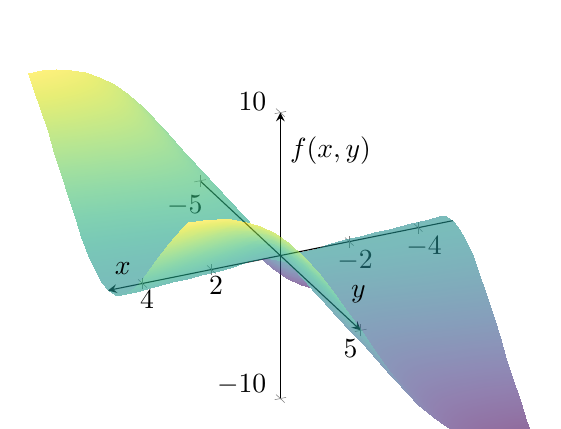
\begin{tikzpicture}
        \begin{axis}[
            xlabel=$x$,
            ylabel=$y$,
            zlabel={$f(x, y)$},
            colormap/viridis,
            view={155}{30},
            axis lines=center,
            width=8cm,
            height=8cm
        ]
        \addplot3[
            surf,
            domain=-5:5,
            domain y=-5:5,
            opacity=0.6,
            shader=interp
        ] {4*x*y^2 / (x^2 + y^2)};
        
        \end{axis}
        \end{tikzpicture}
        \caption{The surface graph shows the limit of the function must be 0, if it exists.}
    \end{figure}
        
    We first observe  that along the line \(x=0\) the function always has value 0 when \(y \neq 0\).
    Likewise, along the line \(y=0\), the function has value 0 provided \(x \neq 0\).
    So if the limit does exist as \((x,y)\) approaches \((0,0)\), the value of the limit must be 0. To see if this is true we apply definition of limit.
    Let \(\epsilon > 0\) be given, but arbitrary. We want to find a \(\delta > 0\) such that
    \[\left|{\frac{4x y^{2}}{x^{2}+y^{2}}}-0\right|<\epsilon \quad \text{whenever} \quad  0 < \sqrt{x^2 + y^2} < \delta\]

    \[\frac{4|x|y^{2}}{x^{2}+y^{2}} \quad \text{whenever} \quad  0 < \sqrt{x^2 + y^2} < \delta   \]

    Since \(y^2 \leq x^2 + y^2\) we have that 
    \[\frac{4|x|y^{2}}{x^{2}+y^{2}} < 4|x| = 4 \sqrt{x^2} \leq 4\sqrt{x^2 + y^2}\]

    So if we chose \(\delta = \epsilon \slash 4\) and let \(0 < \sqrt{x^2 + y^2} < \delta\) we get

    \[\left|\frac{4 x y^2}{x^2+y^2}-0\right| \leq 4 \sqrt{x^2+y^2}<4 \delta=4\left(\frac{\varepsilon}{4}\right)=\varepsilon\]
    It follows from the definition that
    \[\operatorname*{lim}_{(x,y)\rightarrow(0,0)}\frac{4x y^{2}}{x^{2}\,+\,y^{2}}=\,0\]


\end{solution}

\newpage

\begin{example}
    If \(f(x,y) = \frac{x}{y},\) does \( \lim_{(x,y) \to (0,0)}f(x,y)\)  exist?
\end{example}

\begin{solution}
    The domain of \(f\) does not include the y-axis so we do not consider any points \((x,y)\) where \(x=0\) in the approach toward the origin \((0,0)\). Along the x-axis, the value of the function is \( f(x,0) = 0\) for all \(x \neq 0\).
    So if the limit does exist as \((x,y) \to (0,0)\), the value of the limit mus be \(L = 0\). On the other hand, along the line \(y=x\), the value of the function is \(f(x,x) = 1\) for all \(x \neq 0\).
    That is, the function \(f\) approaches the value 1 along the line \(y=x\). This means that for every disk of radius \(\delta\) centered at \((0,0)\), the disk will contain points \((x,0)\) on the x-axis where the value of the function is 0, and also points \((x,x)\) along the line \(y=x\) where the function is 1.
    So no matter how small we choose \(\delta\) as the radius of the disk, there will be points within the disk for which the function values differ by 1. Therefore limit cannot exist because we can take \(\epsilon\) to be any number less than 1 in the limit definition and deny that \(\mathit{L} = 0\) or \(1\), or any other real number.
    The limit does not exist because we have different limiting values along different paths approaching the point \((0,0)\) \hfill \qed

\end{solution}

\subsection{Continuity}

\begin{definition}
    A function \(f(x,y)\) is \textbf{continuous at the point} \((x_0,y_0)\) if
    \begin{enumerate}
        \item \(f\) is defined at \((x_0,y_0)\)
        \item \(\lim_{(x,y) \to (x_0,y_0)}f(x,y)\) exists
        \item \(\lim_{(x,y) \to (x_0,y_0)}f(x,y) = f(x_0,y_0)\) 
    \end{enumerate}
    A function is \textbf{continuous} if it is continuous at every point of its domain.
\end{definition}

\begin{example}
    Show that
    \[f(x, y)= \begin{cases}\frac{2 x y}{x^2+y^2}, & (x, y) \neq(0,0) \\ 0, & (x, y)=(0,0)\end{cases}\]
    is continuous at every point except the origin.
\end{example}

\begin{solution}
    The function \(f\) is continuous at every point \((x,y)\) except \((0,0)\) because its values at point other than  \((0,0)\) are given by a rational function of x and y, and therefore at those points the limiting value is simply obtained by substitution.
    At \((0,0)\), the value of \(f\) is defined but  \(f\) has no limit as \((x,y) \to (0,0)\). The reason is that different paths of approach to the origin can lead to different results, as we can now see.\\
    For every value of m, the function \(f\) has a constant value on the "punctured" line \(y=mx\), \(x\neq0\) because
    \[\left.f(x, y)\right|_{y=m x}=\left.\frac{2 x y}{x^2+y^2}\right|_{y=m x}=\frac{2 x(m x)}{x^2+(m x)^2}=\frac{2 m x^2}{x^2+m^2 x^2}=\frac{2 m}{1+m^2}\]
    Therefore \(f\) has this number as its limit as \((x,y)\) approaches \((0,0)\) along the line:
    \[\lim _{\substack{(x, y) \rightarrow(0,0) \\ \text { along } y=m x}} f(x, y)=\lim _{(x, y) \rightarrow(0,0)}\left[\left.f(x, y)\right|_{y=m x}\right]=\frac{2 m}{1+m^2} \text {. }\]
    The limit changes with each value of slope m. There is therefore no single number we may call the limit of \(f\) as \((x,y)\) approaches the origin. The limit fails to exist, and the function is not continuous at the origin. \hfill \qed

\end{solution}

\newpage

\begin{ruleBox}{Two-Path Test for Nonexistence of a Limit}
    If a function \(f(x,y)\) has different limits along two different pahs in the domain of \(f\) as \((x,y)\) approaches \((x_0,y_0)\), then \(\lim_{(x,y) \to (x_0,y_0)}\) does not exist.

\end{ruleBox}

\begin{example}
    Show that the function 
    \[f(x,y) = \frac{2x^2y}{x^4+y^2}\]
    has no limit as \((x,y)\) approaches \((0,0)\)

\end{example}

\begin{solution}
    The limit cannot be found by direct substitution, whic gives the indeterminite form \(0 \slash 0\).
    We examine the values of \(f\) along parabolic curves that end at \((0,0)\). Along the curve \(y = kx^2\), \(x \neq 0\), the function has the constant value
    \[\left. f(x,y) \right|_{y = kx^2} = \left. \frac{2x^2y}{x^4+y^4} \right|_{y=kx^2} = \lim_{(x,y) \to (0,0)}\left[\left.f(x,y)\right|_{y=kx^2}\right] = \frac{2k}{1+k^2}\]
The limit varies eith the path of approach. If \((x,y)\) approaches \((0,0)\) along the parabola \(y=x^2\) for instance \(k=1\) and the limit is 1. If \((x,y)\) approaches \((0,0)\) along the x-axis, \(k=0\) and the limit is 0. By the two part test, \(f\) has no limit as \((x,y)\) approaches \((0,0)\). \hfill \qed

It can be shown that the function has limit 0 along every straight line path \(y = mx\). This implies that 

\begin{mynote}
Having the same limit along all straight lines approaching \((x_0,y_0)\) does not imply that a limit exists at \((x_0,y_0)\).
\end{mynote}

\end{solution}

\begin{ruleBox}{Continuity of Compositions}
    If \(f\) is continuous at \((x_0,y_0)\) and \(g\) is a single-variable function continuous at \(f(x_0,y_0)\), then the composition \(h = g \circ f\) defined  by \(h(x,y) = g(f(x,y))\) is continuous at \((x_0,y_0)\).

\end{ruleBox}

\subsection{Functions of More Than Two Variables}
The definitions of limit and continuity for functions of two variables and the conclusions about limits and continuity for sums, products, quotients, powers, and compositions all extend to functions of three or more variables. Functions like
\[\ln(x+ y +z) \quad \text{and} \quad \frac{y \sin{z}}{x-1}\]
are continuous throughout their domains and limits like

\[\lim _{P \rightarrow(1,0,-1)} \frac{e^{x+z}}{z^2+\cos \sqrt{x y}}=\frac{e^{1-1}}{(-1)^2+\cos 0}=\frac{1}{2},\]

where \textit{P} denotes the point \((x,y,z)\), may be found by direct substitution.


\subsection{Extreme Values of continuous Functions on Closed, Bounded Sets}

The Extreme Value Theorem states that a function of a single variable that is continuous at every point of a closed, bounded interval \([a,b]\) takes on an absolute maximum value and an absolute minimum value at lest once  in \([a,b]\). The same holds true of a function \(z = f(x,y)\) that is continuous on a closed, bounded set \textit{R} in the plane. The function takes on ab absolute maximum value at some point in \(R\) and an absolute minimum value at some point in \(R\).
The function may take on a maximum or minimum value more then once over \(R\). 

Similar results hold for functions of three or more variables. A continuous function \(w = f(x,yz)\) must take on absolute maximum and minimum values on any closed, bounded set (such as a solid ball or cube, spherical shell, or rectangular solid) on which it is defined.

\section{Partial Derivatives}

\subsection{Partial Derivatives of a Function of Two Variables}

If \((x_0,y_0)\) is a point in the domain of a function \(f(x,y)\), the vertical plane \(y=y_0\) will cut the surface \(z = f(x,y)\) in the curve \(z = f(x,y_0)\).
 
This curve is the graph of the function \(z = f(x,y)\) \(Y = y_0\). The horizontal coordinate in this plane is z; the vertical coordinate is z. The y-value is held constant at \(y_0\), so \(y\) is not a variable.
We define the partial derivative of \(f\) with respect to \(x\) at the point \(x = x_0\). To distinguish partial derivatives from ordinary derivatives we use the symbol \(\partial\) rather than d previously used. In the definition h represents a real number, positive or negative.

\begin{definition}
    The \textbf{partial derivative of \(f(x,y)\) with respect to x at the point \((x_0,y_0)\) is}

    \[\left. \frac{\partial f}{\partial x} \right|_{(x_0, y_0)} = \lim_{h \to 0}\frac{f(x_0+h,y_0)-f(x_0,y_0)}{h}\]

    provided that limit exists.


\end{definition}


The partial derivative of \(f(x,y)\) with respect to x at the point \((x_0,y_0)\) is the same as the ordinary derivative of \(f(x,y_0)\) at the point \(x_0\):

\[\left. \frac{\partial f}{\partial x} \right|_{(x_0, y_0)} = \left. \diff{}{x}f(x,y_0)\right|_{(x_0, y_0)} \].


\begin{definition}
    The \textbf{partial derivative of \(f(x,y)\) with respect to y at the point \((x_0,y_0)\) is}

    \[\left. \frac{\partial f}{\partial y} \right|_{(x_0, y_0)} = \lim_{h \to 0}\frac{f(x_0,y_0+h)-f(x_0,y_0)}{h}\]

    provided that limit exists.


\end{definition}

\subsection{Calculations}

The definitions of \(\diffp{f}{x}\) and \(\diffp{f}{y}\) give us two different ways of differentiating \(f\) at a point: with respect to x in the usual way while treating y as a constant and with respect to y in the usual way while treating x as a constant. As the following examples show, the values oof these partial derivatives are usually different at a given point \((x_0,y_0)\).

\begin{example}
    Find the values of \(\diffp{f}{x}\) and \(\diffp{f}{y}\) at the point \((4,-5)\) if 
    \[f(x,y) = x^2 + 3xy + y -1\].

\end{example}

\begin{solution}
    To find \(\diffp{f}{x}\) we treat y as a constant and differentiate with respect to x:
    \[{\frac{\partial f}{\partial x}}={\frac{\partial}{\partial x}}\,(x^{2}\,+\,3x y\,+\,y\,-\,1)\,=\,2x\,+\,3\cdot1\cdot y\,+\,0\,-\,0\,=\,2x\,+\,3y.\]
    The value of \(\diffp{f}{x}\) at \((4,-5)\) is -7.

    To find  \(\diffp{f}{y}\), we treat x as a constant and differentiate with respect to y:

    \[{\frac{\partial f}{\partial y}}={\frac{\partial}{\partial y}}\left(x^{2}+3x y+y-1\right)\,=\,0\,+\,3\cdot x\cdot1\,+\,1\,-\,0\,=\,3x\,+\,1.\]

    The value of \(\diffp{f}{y}\) at \((4,-5)\) is 13.


\end{solution}


\begin{example}
    Find \(\diffp{z}{x}\) assuming that the equation
    \[yz -\ln z = x+y\]
    defines z as the function of two independent variables x and y and the partial derivative exists.
\end{example}

\begin{solution}
    We differentiate both sides of equation with respect to x, holding y constant and treating z as a differentiable function of x:

    \begin{align*}
        \diffp{}{x}(yz) - \diffp{}{x}\ln z &= \diffp{x}{x} +\diffp{y}{x}\\
        y \diffp{z}{x} - \frac{1}{z} \diffp{z}{x} &= 1 + 0\\
        \left(y - \frac{1}{z}\right) \diffp{z}{z} &= 1\\
        \diffp{z}{x} &= \frac{z}{yz-1}
    \end{align*}
    

\end{solution}

\newpage

\begin{example}
    The plane \(x=1\) intersects the paraboloid \(z = x^2 + y^2\) in a parabola.
    Find the slope of the tangent to the parabola at \((1,2,5)\).
    


    \begin{solution}
        The parabola lies in a plane parallel to yz-plane, and the slope is the value of the partial derivative \(\diffp{z}{y}\) at \((1,2)\):

        \[\left. \diffp{z}{y} \right|_{(1,2)} = \diffp{}{y} \left. \left(x^2 + y^2\right)\right|_{(1,2)} = \left. 2y \right|_{(1,2)} = 4\]

        As a check, we can treat the parabola as the graph of the single-variable function \(z= 1^2 + y^2 \) in the plane \(x = 1\) and ask for the slope at \(y=2\). The slope, 
        calculated now as an ordinary derivative is 

        \[\left. \diff{z}{y}\right|_{y=2} =  \left. \diff{}{y}(1+y^2) \right|_{y=2} =  \left. 2y\right|_{y=2} = 4\]

    \end{solution}

    


\end{example}



\subsection{Functions of more than two Variables}

The definitions of the partial derivatives of functions of more than two independent vari-
ables are similar to the definitions for functions of two variables. They are ordinary deriva-
tives with respect to one variable, taken while the other independent variables are held
constant.


\begin{example}
    If x, y and z are independent variables and

    \[f(x,y,z) = x \sin{(y + 3z)}\]
    
    then

    \begin{align*}
        \diffp{f}{z} &= \diffp{}{z}\left[x \sin{(y + 3z)}\right] = x \diffp{}{z}\sin{(y + 3z)}\\
        &= \cos{(y + 3z)} \diffp{}{z} (y + 3z)\\
        &= 3x\cos{(y + 3z)} 
    \end{align*}
    

\end{example}

\newpage

\begin{example}
    \begin{figure}[!ht]
        \centering
        \resizebox{5cm}{5cm}{%
        \begin{circuitikz}[font=\LARGE]
        
        \draw [ color={rgb,255:red,255; green,0; blue,0} ](6.25,11.5) to[R,l={\normalsize $R_1$}] (10,11.5);
        \draw [ color={rgb,255:red,255; green,0; blue,0} ](6.25,10.25) to[R,l={\normalsize $R_2$}] (10,10.25);
        \draw [ color={rgb,255:red,255; green,0; blue,0} ](6.25,9) to[R,l={\small $R_3$}] (10,9);
        \draw (7.5,5.25) to[battery1] (8.75,5.25);
        \draw (6.25,11.5) to[short] (6.25,9);
        \draw (10,11.5) to[short] (10,9);
        \draw (6.25,10.25) to[short] (5,10.25);
        \draw (5,10.25) to[short] (5,5.25);
        \draw (10,10.25) to[short] (11.25,10.25);
        \draw (11.25,10.25) to[short] (11.25,5.25);
        \draw (8.75,5.25) to[short] (11.25,5.25);
        \draw (5,5.25) to[short] (7.5,5.25);
        
        \end{circuitikz}
        }%
        
        \caption{Parallel connected resistors}
        \label{fig:parallelres}
    \end{figure}

    If resistors of \(R_1\), \(R_2\) and \(R_3\) ohms are connected in parallel to make an R-ohm resistor, the value of R can be found from the equation.

    \[\frac1R =  \frac1R_1 + \frac1R_2 + \frac1R_3\]

    Find the value of \(\frac{\partial R}{\partial R_2}\) when \(R_1 = 30\), \(R_2 = 45\), and \(R_3 = 90\) ohms. 

    \begin{solution}
        
        To find \(\frac{\partial R}{\partial R_2}\), we treat \(R_1\) and \(R_3\) as constants and, using implicit differentiation, differentiate both sides of the equation with respect to \(R_2\):

        
        \begin{align*}
            \frac{\partial}{\partial R_2}\left(\frac{1}{R}\right) &= \left(\frac{1}{R_1} + \frac{1}{R_2} + \frac{1}{R_3}\right)\\
            -\frac{1}{R^2} \frac{\partial R}{\partial R_2} &= 0 - \frac{1}{R_2^2} + 0 \\
            \frac{\partial^2 R}{\partial R_2^2} &= \left(\frac{R}{R_2}\right)^2
        \end{align*}
        
        When \(R_1 = 30, R_2 = 45 \ \text{and} \ R_3 = 90 \) so \(R=15\) and
        \[\frac{\partial R}{\partial R_2} = \frac19\]
    \end{solution}
    Thus at the given values, a small change in the resistance R2 leads to a change in R about
    1/9th as large
\end{example}

\subsection{Partial Derivatives and Continuity}

A function \(f(x,y)\) can have partial derivatives with respect to both x and y at a point without being continuous there. \textcolor{red}{This is different from functions of a single variable, where existence of a derivative implies continuity.} If the partial derivatives of \(f(x,y)\) exist and are continuous throughout a disk centered at \(x_0,y_0\), however, then \(f\) is continuous at \(x_0,y_0\).

\begin{example}
    Let
    \[f(x,y) = \begin{cases}
        0, & xy \neq 0 \\
        1, & xy = 0
    \end{cases}\]

    \begin{enumerate}[label=\textbf{(\alph*)}]
        \item Find the limit of \(f\) as \((x,y)\) approaches \((0,0)\) along the line y = x.
        \item Prove that \(f\) is not continuous at the origin.
        \item Show that both partial derivatives \(\diffp{f}{x}\) and \(\diffp{f}{y}\) exist at the origin.
        
    \end{enumerate}

\end{example}


\begin{solution}
    \begin{enumerate}[label=\textbf{(\alph*)}]
        \item Since \(f(x,y)\) is constantly zero along the line \(y=x\), we have \[\left. \lim_{(x,y) \to (0,0)} f(x,y) \right|_{y=x} = \lim_{(x,y) \to (0,0)} 0 = 0\]
        \item Since \(f(0,0) = 1\), the limit in part (a) is not equal to \(f(0,0)\), which proves \(f\) is not continuous at \((0,0)\).
        \item To find \(\diffp{f}{x}\) at \((0,0)\) we hold y fixed at  \(y=0\). Then \(f(x,y) = 1\) for all x, and the graph of f is a line. The slope of this line a any x is 0. In particular, \(\diffp{f}{x} = 0\) at \((0,0)\). Similarly \(\diffp{f}{y} = 0\) at \((0,0)\).
    \end{enumerate}
\end{solution}


\subsection{Second Order Partial Derivatives}

When we differentiate a function \(f(x,y)\) twice, we produce its second-order derivatives. These derivatives are usually denoted by

\[\diffp[2]{f}{x} \ \text{or} \ f_{xx}, \quad \diffp[2]{f}{y} \ \text{or} \ f_{yy} \],

\[\diffp{f}{{x}{y}} \ \text{or} \ f_{yx}, \quad \diffp{f}{{y}{x}} \ \text{or} \ f_{xy},\]

The defining equations are
\[\diffp[2]{f}{x} = \diffp{}{x}\left(\diffp{f}{x}\right), \quad \diffp{f}{{x}{y}} = \diffp{}{x}\left(\diffp{f}{y}\right)\]


\subsection{The Mixed Derivative Theorem}

\begin{theorem}
    If \fxy abd its partial derivatives \(f_x, f_y, f_{xy}\) and \(f_{yx}\) are defined throughout an open region containign a point \((a,b)\) and are all continuous at  \((a,b)\), then,
    \[f_{xy}(a,b) = f_{yx}(a,b)\]
\end{theorem}

\newpage

\subsection{Differentiability}

The concept of \textit{differentiability} for functions of several variables is more complicated than for single-variable functions because a point in the domain can be approached along more than one path. 
In defining the partial derivatives for a function of two variables, we intersected the surface of the graph with vertical planes parallel to the xz- and yz- planes, creating a curve on each plane, called a \textit{\textbf{trace}}. The partial derivatives were seen as the slopes of two tangent lines to these trace curves at the point on the surface corresponding to the point \((x_0,y_0)\) being approached in the domain. For a differentiable function, it would seem reasonable to to assume that if we were to rotate slightly one of these vertical planes, keeping it vertical but no longer parallel to its coordinate plane, then a smooth trace curve would appear on that plane that would have a tangent line at the point on the surface having a slope differing just slightly from what it was before. 

However, the mere existence of the original partial derivative does not guarantee that result. Just as having a limit in the x- and y-coordinate directions alone does not imply the function itself has a limit at \((x_0,y_0)\), so it is the case that the existence of both partial derivatives is not enough by itself to ensure derivatives exist for trace curves in other vertical planes. 
For the existence of differentiability, a property is needed to ensure that no abrupt change occurs in the function resulting from small changes in the independent variables along any path approaching \((x_0,y_0)\), paths along which \textit{both} variables x and y are allowed to change, rather than just one of them at a time.


In our study of functions of a single variable, we found that if a function \(y= f(x)\) is differentiable at \(x=x_0\), then the change \(\Delta y\) resulting in the change of \(x\) from \(x_0\) to \(x_0 + \Delta x\) is close to the change \(\Delta L\) along the tangent line. That is,

\[\Delta y= f'(x_0)\Delta + \varepsilon \Delta x\]

in which \(\varepsilon \to 0\) as \(\Delta x \to 0\). The extension of this result is what we use to define differentiability for functions of two variables.

\begin{definition}
    A function \(z = f(x,y)\) is \textbf{differentiable at} \((x_0,y_0)\) if \(f_x(x_0,y_0)\) and \(f_y(x_0,y_0)\) exist and 
    \[\Delta z = f_x(x_0,y_0) \Delta x + f_y(x_0,y_0) \Delta y + \varepsilon_1\Delta x + \varepsilon_2\]
    in which each of \(\varepsilon_1, \varepsilon_2 \to 0\) as both \(\Delta x, \Delta y \to 0\). We call \(f\) \textbf{differentiable} if it is differentiable at every point in its domain and its graph is a \textbf{smooth surface}.

\end{definition}


\begin{theorem}
    Suppose that the first partial derivatives of \(f(x,y)\) are defined throughout an open region R containing \((x_0,y_0)\) and that \(f_x\) and \(f_y\) are continuous at \((x_0,y_0)\). Then the change
    \[\Delta z = f(x_0 + \Delta x, y_0 + \Delta y) - f(x_0,y_0)\]
    
    in the value of \(f\) that results from moving from \((x_0,y_0)\) to another point \((x_0 +\Delta x,y_0+ \Delta y)\) in R satisfies an equation of the form
    \[\Delta z = f_x(x_0,y_0) \Delta x + f_y(x_0,y_0) \Delta y + \varepsilon_1\Delta x + \varepsilon_2\]

    in which each of \(\varepsilon_1, \varepsilon_2 \to 0\) as both \(\Delta x, \Delta y \to 0\).
\end{theorem}

\begin{corollary}
    If the partial derivatives \(f_x\) and \(f_y\) of a function \(f(x,y)\) are continuous throughout tan open region R, then \(f\) is differentiable at every point of R. 

\end{corollary}


\textbf{This tells us that a function of two variables is continuous at every point where it is differentiable.
}


\begin{theorem}
    If a function \fxy is differentiable at \((x_0,y_0)\), then f is continuous at \((x_0,y_0)\)
\end{theorem}

\newpage

\section{The chain rule}

The chain rule for functions of a single variable says that when \(w = f(x)\) is a differentiable function of x and \(x= g(t)\) is a differentiable function of t, w is a differentiable function of t and \(\diff{w}{t}\) can be calculated by the formula

\[\diff{w}{t} = \diff{w}{x}\diff{x}{t}\]


\subsection{Functions of Two Variables}

The Chain Rule formula for a differentiable function \(w= f(x,y)\) when \(x = x(t)\) and \(y = y(t)\) are both differentiable functions of t is given by the following theorem.

\begin{theorem}
\textbf{Chain Rule For Functions of one independent Variable and two intermediate Variables}

If \(w = f(x,y)\) is differentiable and if \(x = x(t)\),\(y = y(t)\) are differentiable functions of t, then the composition \(w = f(x(t),y(t))\) is a differentiable function of t and 

\[\diff{w}{t} = f_x(x(t),y(t))x'(t) + f_y(x(t), y(t))y'(t)\]

or

\[\diff{w}{t} = \diffp{f}{x}\diff{x}{t} + \diffp{f}{y}\diff{y}{t}\]


\end{theorem}




\subsection{Functions of Three Variables}

\begin{theorem}
    If \(w = f(x,y,z)\) is differentiable and x, y and z ate differentiable functions of t, then w is a differentiable function of t and
    
    \[\frac{d w}{d t}=\frac{\partial w}{\partial x} \frac{d x}{d t}+\frac{\partial w}{\partial y} \frac{d y}{d t}+\frac{\partial w}{\partial z} \frac{d z}{d t}\]

\end{theorem}

\subsection{Functions Defined on Surfaces}

\begin{theorem}
    Chain Rule for two independent Variables and three intermediate Variables

    Suppose that \(w = f(x,y,z)\), \(x= g(r,s)\), \(y= h(r,s)\) and \(z= k(r,s)\). If all four
    functions are differentiable, then w has partial derivatives with respect to r and s,
    given by the formulas.

    \[\begin{aligned}
        & \frac{\partial w}{\partial r}=\frac{\partial w}{\partial x} \frac{\partial x}{\partial r}+\frac{\partial w}{\partial y} \frac{\partial y}{\partial r}+\frac{\partial w}{\partial z} \frac{\partial z}{\partial r} \\
        & \frac{\partial w}{\partial s}=\frac{\partial w}{\partial x} \frac{\partial x}{\partial s}+\frac{\partial w}{\partial y} \frac{\partial y}{\partial s}+\frac{\partial w}{\partial z} \frac{\partial z}{\partial s}
        \end{aligned}\]

\end{theorem}



\subsection{Implicit Differentiation Revisited}

Suppose that

\begin{enumerate}
    \item The function \(F(x,y)\) is differentiable and
    \item The equation \(F(x,y) = 0\) define y implicitly as a differentiable function of x, say \(y= h(x)\).

\end{enumerate}


Since \(w = F(x,y) = 0\), the derivative \(\diff{w}{x}\) must be zero. Computing the derivative we Find

\begin{align*}
    0 &= \diff{w}{x} = F_x \diff{x}{x} + F_y \diff{y}{x} \\
    &= F_x+ F_y \diff{y}{x}    
\end{align*}
 
If \(F_y \diffp{w}{y} \neq 0\) we can solve this equation for \(\diff{y}{x}\) to get

\[\diff{y}{x} = - \frac{F_x}{F_y}\]

\begin{theorem}
    Suppose that \(F(x,y)\) is differentiable and that the equation \(F(x,y) = 0\) defines y as a differentiable function of x. Then at any point where \(F_y \neq 0\)

    \[\diff{y}{x} = - \frac{F_x}{F_y}\]
\end{theorem}


\subsubsection{Three Variables}
The result in the theorem is easily extended to three variables. Suppose that the equation \(F(x,y,z) = 0\) defines the cariable z implicitly as a function \(z = f(x,y)\). Then for all \((x,y)\) in the domain of f, we have \(F(x,y, f(x,y))\).
Assuming that F and f are differentiable functions, we can use the chain rule to differentiate the equation \(F(x,y,z) = 0\) with respect to independent variable x:

\[\begin{aligned}
    0 & =\frac{\partial F}{\partial x} \frac{\partial x}{\partial x}+\frac{\partial F}{\partial y} \frac{\partial y}{\partial x}+\frac{\partial F}{\partial z} \frac{\partial z}{\partial x} \\
    & =F_x \cdot 1+F_y \cdot 0+F_z \cdot \frac{\partial z}{\partial x}
    \end{aligned}\]

so

\[F_x + F_z \diffp{z}{x} = 0\]
A similar calculation for differentiating with respect to the independent variable y gives

\[F_y + F_z \diffp{z}{y} = 0\].

Whenever \(F_z \neq 0\), we can solve these last two equations for the partial derivatives of \(z= f(x,y)\) to obtain

\begin{note}

\[\diffp{z}{x} = - \frac{F_x}{F_z} \quad \text{and} \quad \diffp{z}{y} = - \frac{F_y}{F_z}\]

\end{note}


\subsection{Functions of many Variables}

In general, suppose that \(w = f(x,y,z, \dots, \mathbf{v})\) is a differentiable function of intermediate variables \(x,y,z, \dots, \mathbf{v}\) and the \(x,y,z, \dots, \mathbf{v}\) differentiable functions of the independent variables \(p,q, \dots, t\) hen w is a differentiable
function of the variables p through t, and the partial derivatives of w with respect to these variables are given by equations of the form

\[\frac{\partial w}{\partial p}=\frac{\partial w}{\partial x} \frac{\partial x}{\partial p}+\frac{\partial w}{\partial y} \frac{\partial y}{\partial p}+\cdots+\frac{\partial w}{\partial \boldsymbol{v}} \frac{\partial \boldsymbol{v}}{\partial p}\]


The other equations are obtained by replacing p by q, . . . , t, one at a time. One way to remember this equation is to think of the right-hand side as the dot product of two vectors with components

\[\left(\frac{\partial w}{\partial x}, \frac{\partial w}{\partial y}, \dots, \frac{\partial w}{\partial \mathbf{v}}\right) \quad \text{and} \quad \left(\frac{\partial x}{\partial p}, \frac{\partial y}{\partial p}, \dots, \frac{\partial \mathbf{v}}{\partial p}\right)\]


\section{Directional Derivatives and Gradient Vectors}

\begin{definition}
    The \textbf{derivative of f at \(P_0(x_0,y_0)\) in the direction of the unit vector \(u = u_1i + u_2j\)} is the numbers
    \[\left(\diff{f}{s}\right)_{\mathbf{u}, P_0} = \lim_{s \to 0}\frac{f(x_0+ su_1, y_0 + su_2) - f(x_0,y_0)}{s}\]
    provided the limit exists.
\end{definition}

The \textbf{directional derivative} defined by the equation is also denoted by
\[D_uf(P_0) \quad \text{or} \quad D_uf|_{P_0} \]

\begin{example}
    Using the definition, find the derivative of
    \[f(x,y)= x^2 + y^2\]
    at \(P_0(1,2)\) in the direction of the unit vector \(\mathbf{u} = \frac{1}{\sqrt{2}}i + \frac{1}{\sqrt{2}}j \)
\end{example}

\begin{solution}
    \[\begin{aligned}
        &\begin{aligned}
        \left(\frac{d f}{d s}\right)_{\mathbf{u}, P_0} & =\lim _{s \rightarrow 0} \frac{f\left(x_0+s u_1, y_0+s u_2\right)-f\left(x_0, y_0\right)}{s} \\
        & =\lim _{s \rightarrow 0} \frac{f\left(1+s \cdot \frac{1}{\sqrt{2}}, 2+s \cdot \frac{1}{\sqrt{2}}\right)-f(1,2)}{s} \\
        & =\lim _{s \rightarrow 0} \frac{\left(1+\frac{s}{\sqrt{2}}\right)^2+\left(1+\frac{s}{\sqrt{2}}\right)\left(2+\frac{s}{\sqrt{2}}\right)-\left(1^2+1 \cdot 2\right)}{s} \\
        & =\lim _{s \rightarrow 0} \frac{\left(1+\frac{2 s}{\sqrt{2}}+\frac{s^2}{2}\right)+\left(2+\frac{3 s}{\sqrt{2}}+\frac{s^2}{2}\right)-3}{s} \\
        & =\lim _{s \rightarrow 0} \frac{\frac{5s}{\sqrt{2} + s^2}}{\sqrt{2}+s^2}=\lim _{s \rightarrow 0}\left(\frac{5}{\sqrt{2}}+s\right)=\frac{5}{\sqrt{2}} .
        \end{aligned}\\
        \end{aligned}
        \]
    The rate of change in the direction of u is \(\frac{5}{\sqrt{2}}\)
\end{solution}

\subsection{Calculation and Gradients}

We now develop an efficient formula to calculate the directional derivative for a differen-
tiable function ƒ. We begin with the line

\[x = x_0 + su_1 \quad y = y_0 + su_2\]

through \(P(x_0,y_0)\) parametrized with the arc lenght parrameter s increasing in the direction of the unit vector \(u = u_1 \hat{i} + u_2 \hat{j}\) Then by the chain rule we find

\[\begin{aligned}
    \left(\frac{d f}{d s}\right)_{\mathbf{u}, P_0} & =\left.\frac{\partial f}{\partial x}\right|_{P_0} \frac{d x}{d s}+\left.\frac{\partial f}{\partial y}\right|_{P_0} \frac{d y}{d s} \quad \text { Chain Rule for differentiable } f \\
    & =\left.\frac{\partial f}{\partial x}\right|_{P_0} u_1+\left.\frac{\partial f}{\partial y}\right|_{P_0} u_2 \quad \begin{array}{l}
    \text { From Eqs. (2), } d x / d s=u_1 \\
    \text { and } d y / d s=u_2
    \end{array} \\
    & =\underbrace{\left[\left.\frac{\partial f}{\partial x}\right|_{P_0} \mathbf{i}+\left.\frac{\partial f}{\partial y}\right|_{P_0} \mathbf{j}\right.}_{\text {Gradient of } f \text { at } P_0} \cdot \underbrace{\left[u_1 \mathbf{i}+u_2 \mathbf{j}\right]}_{\text {Direction } \mathbf{u}} .
    \end{aligned}\]




\begin{definition}
    The \textbf{gradient vector} or \textbf{gradient} of \fxy is the vector
    \[\nabla f = \diffp{f}{x} \hat{i} + \diffp{f}{y} \hat{j} \]
    The value of the gradient vector obtained by evaluating the partial derivatives at a point \(P_0 f(x_0,y_0z)\)
    
\end{definition}


\begin{definition}
    If \fxy is differentiable in an open region containing \(P_0(x_0,y_0)\), then
    \[\left(\diff{f}{s}\right)_{\mathbf{u},P_0} = \nabla \left. \right|_{P_0 \cdot \mathbf{u}}\]

    the dot product of the gradient \(\nabla f\) at \(P_0\) with the vector \textbf{u}. In brief \(D_u f = \nabla f \cdot \mathbf{u}\)

\end{definition}


\subsection{Gradients and tangents to level Curves}

If a differentiable function \fxy has a constant value c along a smooth curve \(\mathbf{r} = g(t)\mathbf{i} + h(t) \mathbf{j}\) then \(f(g(t),h(t)) = c\). Differentiating both sides of this equation with respect to t leads to the equations.


\begin{align*}
    \diff{}{t}f(g(t),h(t)) &= \diff{}{t}(c) \\[1\baselineskip]
    \diffp{f}{x} \diff{g}{t} + \diffp{f}{y} \diff{h}{t} &= 0 \\[1\baselineskip]
    \underbrace{\left(\diffp{f}{x}\mathbf{i} + \diffp{f}{y}\mathbf{j}\right)}_{\nabla f} \cdot \underbrace{\left(\diff{g}{t}\textbf{i} + \diff{h}{t}\mathbf{j}\right)}_{\diff{r}{t}} &= 0\\[1\baselineskip]
\end{align*}

\begin{mynote}
    At every point \((x_0,y_0)\) in the domain of a differentiable function \fxy, the gradient of f is normal to the curve through \((x_0,y_0)\)
\end{mynote}




\begin{ruleBox}{Tangent line to a level Curve}
    \[f_x(x_0,y_0)(x-x_0) + f_y(x_0,y_0)(y-y_0) = 0\]
\end{ruleBox}



\begin{ruleBox}{Algebra Rules for Gradients}

    \begin{enumerate}
        \item Sum Rule: \quad \(\nabla (f + g) = \nabla f + \nabla g\)
        \item Difference Rule \quad \(\nabla (f - g) = \nabla f - \nabla g\)
        \item Constant Multiple Rule: \quad \(\nabla (kf) = k \nabla f\)
        \item Product Rule: \quad \(\nabla(fg) = f \nabla g  + g \nabla f\)
        \item  Quotient Rule: \quad \(\nabla \left( \frac{f}{g}\right) = \frac{g \nabla f - f \nabla g}{g^2}\)
    \end{enumerate}

    
\end{ruleBox}


\subsection{The Chain Rule }

\begin{ruleBox}{The Derivative Along A Path}

    \[\diff{}{t}f(r(t))= \nabla f(r(t)) r'(t)\]
    
\end{ruleBox}


\section{Tangent Planes and Differentials}

\begin{definition}
    The \textbf{tangent plane} to the level surface \(f(x,y,z)=C\) of a differentiable function f at a point \(P_0\) where the gradient is not zero is the plane through \(P_0\) normal to \(\nabla f |_{P_0}\). \\
    The \textbf{normal line} of the surface at \(P_0\) is the line through \(P_0\) parallel to \(\nabla f |_{P_0}\)

\end{definition}


\begin{mynote}
    \textcolor{blue}{\textbf{Tangent Plane to \(f(x,y,z) = c\) at \(P_0(x_0,y_0,z_0)\)}}
    \[f_x(P_0)(x-x_0) + f_y(P_0)(y-y_0) + f_z(P_0)(z-z_0)=\]
    \textcolor{blue}{\textbf{Normal Line to \(f(x,y,z) = c\) at \(P_0(x_0,y_0,z_0)\)}}
    \[x = x_0 + f_x(P_0)t, \quad y = y_0 + f_y(P_0)t, \quad z = z_0 + f_z(P_0)t \]

\end{mynote}



\begin{mynote}
    \textcolor{blue}{\textbf{Plane Tangent to a Surface \(z = f(x,y) at (x_0,y_0,f(x_0,y_0))\)}}
    \[f_x(P_0)(x-x_0) + f_y(P_0)(y-y_0) = (z-z_0)\]

\end{mynote}

\subsection{Estimating Change in f in a Direction u }

\begin{mynote}
    To estimate the change in the value of a differentiable function f when we move a small distance ds from a point \(P_0\) in a particular direction \textbf{u}, use the formula

    \[\mathrm{d}f = (\nabla f|_{P_0} \cdot \mathbf{u}) ds\]

\end{mynote}


\subsection{How to Linearize a Function of Two Variables }

\begin{definition}
    The \textbf{linearization of a function \fxy at a point \((x_0,y_0)\)} where f is differentiable is the function
    \[L(x,y) = f(x_0,y_0) + f_x(x_0,y_0)(x-x_0) + f_y(x_0,y_0)(y-y_0).\]
    The approximation
    \[f(x,y) \approx L(x,y)\]
\end{definition}

\begin{definition}
    If we move from \((x_0,y_0)\) to a point \((x_0 + dx, y_0+ dy)\) nearby the resulting change 
    \[df = f_x(x_0,y_0)dx + f_y(x_0,y_0) dy\]
    in the linearization of f is called the \textbf{total differential of f}
\end{definition}

\subsection{Functions of More Than Two Variables}

The linearization of \(f(x,y,z)\) at a point \(P_0(x_0,y_0,z_0)\) is 
\[L(x,y,z) = f(P_0) + f_x(P_0)(x-x_0) + f_y(P_0)(y-y_0) + f_z(P_0)(z-z_0)\]


\section{Extreme Values and Saddle Points}



\begin{figure}[h]
    \centering
    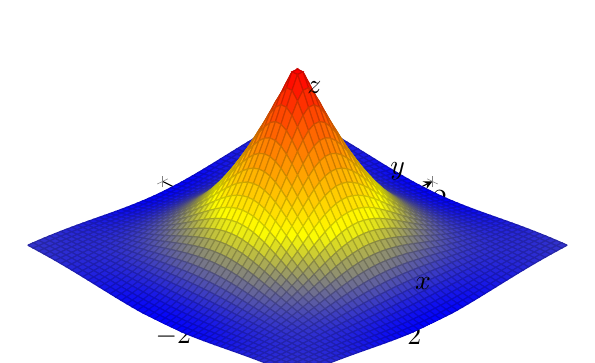
\begin{tikzpicture}
    \begin{axis}[
        xlabel=$x$,
        ylabel=$y$,
        zlabel=$z$,
        domain=-2:2,
        y domain=-2:2,
        colormap/hot,
        samples=50,
        axis lines=center,
        view={45}{45}
    ]
    \addplot3 [surf] {cos(deg(x))*cos(deg(y))*exp(-sqrt(x^2 + y^2))};

    \end{axis}
    \end{tikzpicture}
    \caption{Surface plot of $f(x,y) = \cos(x)\cos(y)e^{-\sqrt{x^2 + y^2}}$ with additional points}
\end{figure}


\subsection{Derivative Test for Local Extrema}

\begin{definition}
    Let \fxy be defined on region R containing the point \((a,b)\). Then
    \begin{enumerate}
        \item \(f(a,b)\) is a \textbf{local maximum} value of f if \(f(a,b) \geq f(x,y)\) for all domain points \((x,y)\) is an open disk centered at \((a,b)\).
        \item \(f(a,b)\) is a \textbf{local minimum} value of f if \(f(a,b) \leq f(x,y)\) for all domain points \((x,y)\) is an open disk centered at \((a,b)\).
    \end{enumerate}
\end{definition}


\begin{theorem}
    If \fxy has a local maximum or minimum value at an interior point \((a,b)\) of its domain and if the first partial derivatives exist there then \(f_x(a,b)=0\) and  \(f_y(a,b)=0\).
\end{theorem}


\begin{definition}
    An interior point of the domain of a function \(f(x,y)\) where both \(f_x\) and  \(f_y\) are zero or where one or both of \(f_x\) and  \(f_y\) do not exist is a \textbf{critical point } of \(f\).
\end{definition}


\begin{definition}
    a differentiable function \fxy has a \textbf{saddle point} at a critical point \((a,b)\) if in every open disk centered at \((a,b)\) there are domain points \((x,y)\) where \(f(x,y) > f(a,b)\) and domain points \((x,y)\) where \(f(x,y) < f(a,b)\). The corresponding point \((a, b, f(a,b))\) on the surface \(z = f(x,y)\) is called a saddle point.
\end{definition}



\begin{example}
    Find the local extreme values of \(f(x,y) = x^2 + y^2 -4y +9\)
\end{example}

\begin{solution}
    The domain of \(f\) is the entire plane and the partial derivatives \(f_x = 2x\) and \(f_y = 2y -4\) exist everywhere. Therefore local extreme values can occur only where

    \[f_x = 2x = 0 \quad \text{and} \quad f_y = 2y-4 = 0\] 
    The only possibility is the point \((0,2)\), where the value of \(f\) is 5. Since \(f(x,y) = x^2 + y^2 -4y +9\)  is never less than 5, we see that the critical point \((0,2)\) gives a local minimum.

\end{solution}

\begin{example}
    Find the local extreme values of \(f(x,y) = y^2 - x^2\)

    \begin{solution}
        The domain of f is the entire plane and the partial derivatives \(f_x = -2x\) and \(f_y = 2y\) exist everywhere. Therefore local extrema can only occur only at the origin \((0,0)\) where \(f_x = 0\) and \(f_y = 0\).
        Along the positive x-axis, \(f\) has the value \(f(x,0) = -x^2 < 0\); along the positive y-axis f has the value \(f(0,y) = y^2 > 0\). Therefore, every open disk in the xy-plane centered at the origin contains points where the function is postive and negative. The function has a saddle point at the origin and no local extreme values.
    \end{solution}

\end{example}

\begin{theorem}
    Suppose that \fxy and its first and second partial derivatives are continuous throughout a disk centered at \((a,b)\) and that \(f_x(a,b) = f_y(a,b)=0\). Then
    \begin{enumerate}
        \item \(f\) has a \textbf{local maximum} at \((a,b)\) if \(f_{xx} < 0\) and \(f_{xx}f_{yy}-f_{xy}^2 > 0\) at \((a,b)\)
        \item \(f\) has a \textbf{local minimum} at \((a,b)\) if \(f_{xx} > 0\) and \(f_{xx}f_{yy}-f_{xy}^2 > 0\) at \((a,b)\)
        \item \(f\) has a \textbf{saddle point} at \((a,b)\) if  \(f_{xx}f_{yy}-f_{xy}^2 < 0\) at \((a,b)\)
        \item \textbf{the test is inconclusive at}  \((a,b)\) \(f_{xx}f_{yy}-f_{xy}^2 = 0\) at \((a,b)\)
    \end{enumerate}
\end{theorem}

The expression \(f_{xx}f_{yy}-f_{xy}^2 = 0\) is called the \textbf{discriminant} or \textbf{Heissian} of \(f\).

\[f_{xx}f_{yy}-f_{xy}^2  = \begin{vmatrix} f_{xx} & f_{xy} \\ f_{xy} & f_{yy} \end{vmatrix}\]

Theorem 11 says that if the discriminant is positive at the point (a, b), then the surface
curves the same way in all directions: downward if \(f_{xx}\), giving rise to a local maxi-
mum, and upward if  \(f_{xx}\) , giving a local minimum. On the other hand, if the discrimi-
nant is negative at (a, b), then the surface curves up in some directions and down in others,
so we have a saddle point

\subsection{Absolute maxima and minima On Closed Bounded Regions}


We organize the search for absolute extrema of a continuous function \(f(x,y)\) on a closed bounded region R by following these steps:

\begin{enumerate}
    \item List the inerior points of R where \(f\) may have a local maxima and minima and evaluate \(f\) at these points. These are the critical points of \(f\) in R.
    \item List the boundary points of R where \(f\) may have a local maxima and minima and evaluate \(f\) at these points. 
    \item Compare the values of \(f\) at the critical points and boundary points to determine the absolute maxima and minima of \(f\) in R.
\end{enumerate}

\section{Lagrange Multipliers}

\subsection{Constrained Maxima and Minima}

\begin{example}
    Find the point \(p(x,y,z)\) on the plane \(2x + y  -z -5 = 0\) that is closest to the origin.

    \begin{solution}
        Since the problem asks us to find the minimum value of the function
        \[\left|\overrightarrow{OP}\right| = \sqrt{(x-0)^2 + (y-0)^2 + (z- 0)^2} = \sqrt{x^2 + y^2 + z^2}  \]



        subject to the constraint that
        \[2x + y -z - 5 =0.\]

        Since \(\left|\overrightarrow{OP}\right|\) has a minimum value wherever the functipn
        \[f(x,y,z) = x^2 + y^2 + z^2\]
        has a minimum value, we may solve the problem by finding the minimum value of \(f(x,y,z)\) subject to the constraint \(2x + y - z -5 = 0\). If we regard x and y as independent variables in this equation and write z as
        \[z = 2x + y - 5\]

        our problem reduces to one of finding the points \((x,y)\) at which the function
        \[h(x,y) = f(x,y, 2x + y -5) = x^2 + y^2 + (2x + y -5)^2\]

        has its minimum value or values. Since the domain of h is the entire xy-plane, the first derivative test tells us that any minima that h might have must occur at points where
        \[h_x = 2x + 2(2x+ y -5)(2) = 0, \quad h_y = 2y + 2(2x+y-5) = 0\]
        This leads to 
        \[10x + 4y = 20, \quad 4x + 4y = 10,\]
        which has the solution

        \[x = \frac{5}{3}, \quad y = \frac56\]

        We may apply a geometric argumet together with the second derivative test to show that these values minimize h. The z-coordinate of the corresponding point on the plane \(z = 2x + y -5\) is \(z = -\frac56\)

        Therefore, the point we seek is 
        \[\text{Closest Point:} \quad P \left(\frac53,\frac56,-\frac56\right)\]
        The distance from the origin is \(\frac{5}{\sqrt{6}}\)





    \end{solution}

   
\end{example}




\begin{example}
    Find the points on the hyperbolic cylinder \(x^2 - z^2 -1 = 0\) that are closest to the origin.

    \begin{solution}
        We seek the points on the hyperbolic cylinder closest to the origin. These are the points whose coordinates minimize the value of the function
        \[f(x,y,z) = x^2 + y^2 + z^2\]
        subject to the constraint that \(x^2 - z^2 -1 = 0\). If we regard x and y as independent variables inn the contraint equation, Then
        \[z^2 = x^2 -1\]

        and the values of \(f(x,y,z) = x^2 + y^2 + z^2 \) on the cylinder are given by the function
         \[h(x,y) = x^2 + y^2 + (x^2 -1) = 2x^2 + y^2 -1\].

         To find the points on the cylinder whose coordinates minimize f, we look for the points in the xy-plane whose coordinates minimize h. The only extreme values of h occurs where
         \[h_x = 4x = 0, \quad h_y = 2y = 0\]
         that is at the point \((0,0)\). But there are no points on the cylinder where both x and y are zero. We can avoid this problem by treating y  and z as independent variables and express x in terms of y and z as

          \[x^2 = z^2 +1\]
          With this substitution \(f(x,y,z) = x^2 + y^2 + z^2 \) becomes 
          \[k(x,y) = (z^2 +1) + y^2 + z^2 \]

          and we look for the points where k takes on its smallest value. The domain of k in the yz-plane now matches the domain from which we select the y- and z-coordinates of the points (x, y, z) on the cylinder. Hence, the points that minimize k in the plane will have corresponding points on the cylinder. The smallest values of k occur where
          \[k_y = 2y = 0 \quad k_z = 4z = 0\],

          or where \(y = z = 0\). This leads to 
          \[x^2 = z^2 +1 = 1, \quad x = \pm 1.\]

          The corresponding points on the cylinder are \(\pm 1, 0, 0\)

        \end{solution}
        \begin{solution}
            Another way to find the points on the cylinder closest to the origin is to imagine a small sphere centered at the origin expanding like a soap bubble until it just touches the cylinder. At each point of contact, the cylinder and the sphere have the same tangent plane and the normal line. Therefore, if sphere and cylinder are represented as the level surfaces obtained by setting
            \[f(x,y,z) = x^2 + y^2 + z^2 -a^2 \quad \textrm{and} \quad g(x,y,z) = x^2 - z^2 -1\]
            equal to 0, then the gradients \(\nabla f\) and \(\nabla g\) will be parallel where the surfaces touch . At any point of contact, we should therefore be able to find a scalar \(\lambda\)such that
            \[\nabla f = \lambda \nabla g\],
            or
            \[2x\mathbf{i} + 2y\mathbf{j} + 2z\mathbf{k} = \lambda (2x\mathbf{i} -2z \mathbf{k} )\]
            Thus the coordinates x,y and z of any point tangency will have to satisfy the three scalar equations
            \[2x = 2\lambda x, \quad 2y = 0, \quad 2z = -2 \lambda z.\]

            \[2\lambda = 2 \quad \lambda =1\]
            The points on the cylinder closest to the origin are the points \((\pm 1, 0,0)\).



        \end{solution}

        
\end{example}


\subsection{The Method of Lagrange Multipliers}

\begin{ruleBox}{The Orthogonal Gradient Theorem}

    Suppose that \(f(x,y,z)\) is differentiable in a region whose interior contains a smooth curve

    \[C: \hspace*{0.5em} \mathbf{r}(t) = x(t)\mathbf{i} + y(t)\mathbf{j} + z(t)\mathbf{k}\]

    If \(P_0\) is a point on C where \(f\) has a local maximum or minimum relative to its values on C, then \(\nabla f\) is orthogonal to C at \(P_0\).
    
\end{ruleBox}

\begin{corollary}
    At the points on the smooth curve \(\mathbf{r}(t) = x(t)\mathbf{i} + y(t)\mathbf{j}\) where a differentiable function \(f(x,y)\) takes on its local maxima and minima relative to its values of the curve, \(\nabla f \cdot r' = 0\).


\end{corollary}


\begin{ruleBox}{The Method of Lagrange Multipliers}
    
    Suppose that \( f(x,y,z) \) and \( g(x,y,z) \) are differentiable, and \( \nabla g \neq 0 \) when \( g(x,y,z) = 0 \).
    To find the local maximum and minimum values of f subject to the constraint \(g(x,y,z) = 0\), find the values of x,y,z and \(\lambda\) that 
    simultaneously satisfy the equations
    \[\nabla f = \lambda \nabla g \quad \text{and} \quad g(x,y,z) = 0.\]

    For functions of two independent variables, the condition is similar, but without the variable z.

    
\end{ruleBox}



\subsection{Lagrange Multipliers with Two Constraints}

Many problems require us to find the extreme values of a differentiable function \(f(x,y,z)\) whose variabless are subject to two constraints. If the constraints are 

\[g_1(x,y,z) = 0 \quad \text{and} \quad g_2(x,y,z) = 0\]

and \(g_1\) and \(g_2\) are differentiable, with \(\nabla g_1\) not parallel to \(\nabla g_2\), we find the constrained local maxima and minima of \(f\) by introducing two Lagrange multipliers \(\lambda\) and \(\mu\).
That is, we locate the points \(P(x,y,z)\), where f takes on its constrained extreme values by finding the values of x,y,z,\(\lambda\) and \(\mu\) that simultaneously satisfy three equations


\begin{mynote}
    \[\nabla f = \lambda \nabla g_1 + \mu \nabla g_2, \quad g_1(x,y,z) = 0, \quad  g_2(x,y,z) = 0 \]
    
\end{mynote}




\end{document}